\documentclass{article}
\usepackage[warn]{mathtext}
\usepackage[utf8]{inputenc}
\usepackage[russian]{babel}
\usepackage{mathtools}
\usepackage[left=2cm,right=2cm,top=1cm,bottom=2cm,bindingoffset=0cm]{geometry}
\renewcommand{\baselinestretch}{1.5}
\usepackage{amsmath}
\usepackage{graphicx}
\usepackage{amssymb}
\usepackage{tikz}
\usepackage{ wasysym }
\usepackage{mathtools}
\usepackage{tabto}
\usepackage[export]{adjustbox}
\DeclarePairedDelimiter\ceil{\lceil}{\rceil}
\DeclarePairedDelimiter\floor{\lfloor}{\rfloor}
\DeclareSymbolFont{T2Aletters}{T2A}{cmr}{m}{it}

\title{Documentation}
\author{Мирославский Прохор, Лапшин Никита, Бажан Денис}
\date{}

\begin{document}

\maketitle

\section{Описание проекта}
Мы реализовали модель мотоцикла с настраиваемыми физическими параметрами такими как масса, жёсткость рессор, поле, в котором он двигается и др. и благодаря мультимедийной библиотеке SFML построили трассу для наглядной демонстрации выполненной работы. Для построения движения использовался метод Рунге-Кутта:\\
Есть s этапов, на каждом из которых происходит вызов функции f() с каким-то параметром.\\
Первый шаг заключается в вызове функции x(t) – изначальном состояние динамической системы.\\
Последующие шаги являются вызовом функции f, в которых записана некоторая линейная комбинация результатов, полученных на предыдущих шагах.\\
\section{Подготовка}
Необходимо установить мультимедийную библиотеку SFML и прочитать документацию по использованию функций, применяемых в работе.
\section{Описание файлов}
CMakeLists.txt - сборочный файл программы\\
main.h - подключение графичесой библиотеки\\
main.cpp - реализация всей графической составляющей программы\\
Vector.h - описание структуры для работы с векторами\\
Vector.cpp - реализация операций с векторами\\
bike.h - описание структур всех частей мотоцикла\\
bike.cpp - реализация всей физики мотоцикла и его движения по графике\\
\\ \\ \\ \\ \\
\section{Соотношение классов}
\begin{figure}[h]
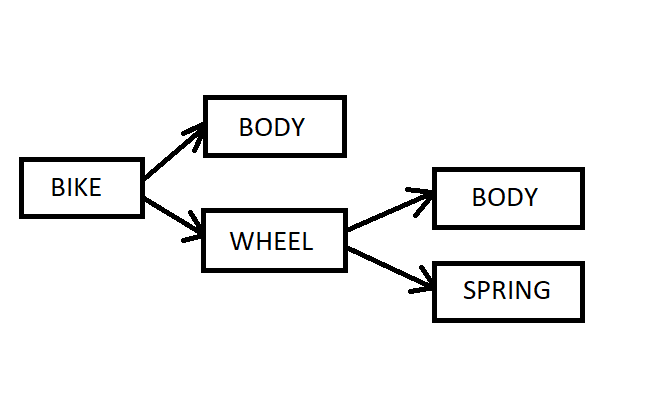
\includegraphics[]{Безымянный.png}
\centering
\end{figure}\\
\end{document}
